\tikzset{every picture/.style={line width=0.75pt}} %set default line width to 0.75pt        

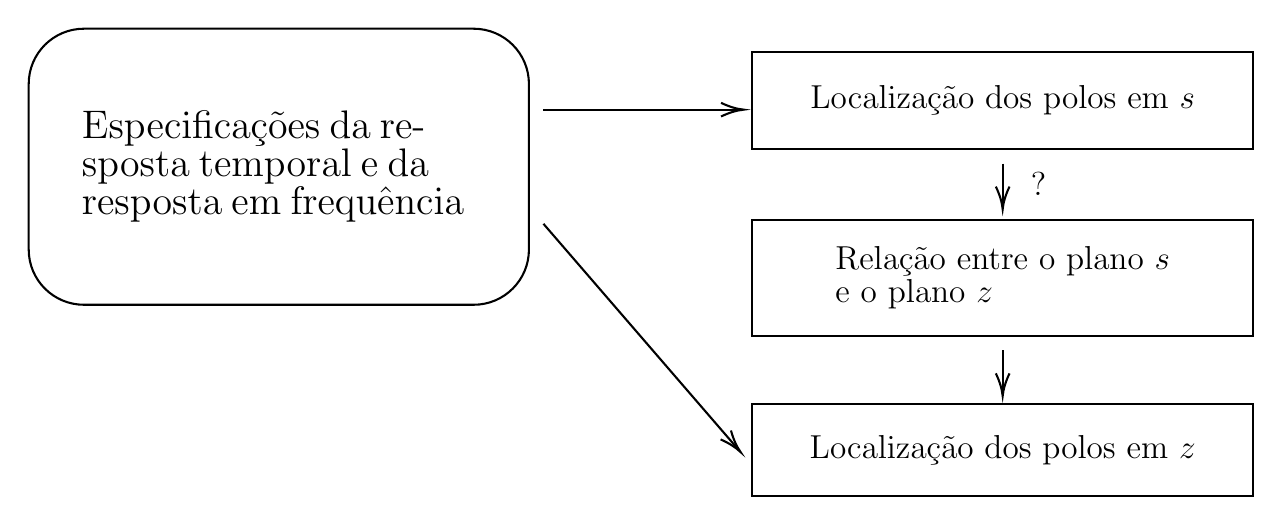
\begin{tikzpicture}[x=0.75pt,y=0.75pt,yscale=-1,xscale=1]
%uncomment if require: \path (0,300); %set diagram left start at 0, and has height of 300

%Rounded Rect [id:dp5431796487964364] 
\draw   (22.5,60.6) .. controls (22.5,45.91) and (34.41,34) .. (49.1,34) -- (236.9,34) .. controls (251.59,34) and (263.5,45.91) .. (263.5,60.6) -- (263.5,140.4) .. controls (263.5,155.09) and (251.59,167) .. (236.9,167) -- (49.1,167) .. controls (34.41,167) and (22.5,155.09) .. (22.5,140.4) -- cycle ;
%Shape: Rectangle [id:dp3399561056052016] 
\draw   (371,45) -- (612.5,45) -- (612.5,92) -- (371,92) -- cycle ;
%Shape: Rectangle [id:dp6770621584559042] 
\draw   (371,126) -- (612.5,126) -- (612.5,182) -- (371,182) -- cycle ;
%Shape: Rectangle [id:dp6731969801823008] 
\draw   (371,215) -- (612.5,215) -- (612.5,259) -- (371,259) -- cycle ;
%Straight Lines [id:da37955603530403326] 
\draw    (491.75,99) -- (491.75,119) ;
\draw [shift={(491.75,121)}, rotate = 270] [color={rgb, 255:red, 0; green, 0; blue, 0 }  ][line width=0.75]    (10.93,-3.29) .. controls (6.95,-1.4) and (3.31,-0.3) .. (0,0) .. controls (3.31,0.3) and (6.95,1.4) .. (10.93,3.29)   ;

%Straight Lines [id:da210617530005335] 
\draw    (491.75,189) -- (491.75,209) ;
\draw [shift={(491.75,211)}, rotate = 270] [color={rgb, 255:red, 0; green, 0; blue, 0 }  ][line width=0.75]    (10.93,-3.29) .. controls (6.95,-1.4) and (3.31,-0.3) .. (0,0) .. controls (3.31,0.3) and (6.95,1.4) .. (10.93,3.29)   ;

%Straight Lines [id:da873322200776687] 
\draw    (270.5,73) -- (365,73) ;
\draw [shift={(367,73)}, rotate = 180] [color={rgb, 255:red, 0; green, 0; blue, 0 }  ][line width=0.75]    (10.93,-3.29) .. controls (6.95,-1.4) and (3.31,-0.3) .. (0,0) .. controls (3.31,0.3) and (6.95,1.4) .. (10.93,3.29)   ;

%Straight Lines [id:da09629763731188756] 
\draw    (270.5,128) -- (364.19,236.49) ;
\draw [shift={(365.5,238)}, rotate = 229.18] [color={rgb, 255:red, 0; green, 0; blue, 0 }  ][line width=0.75]    (10.93,-3.29) .. controls (6.95,-1.4) and (3.31,-0.3) .. (0,0) .. controls (3.31,0.3) and (6.95,1.4) .. (10.93,3.29)   ;


% Text Node
\draw (143,100.5) node  [align=left, text width=5cm] {\Large Especificações da resposta temporal e da resposta em frequência};
% Text Node
\draw (491.75,68.5) node  [align=left] {{\large Localização dos polos em $ s $}};
% Text Node
\draw (491.75,154) node  [align=left] {{\large Relação entre o plano $s $}\\{\large e o plano $z $}};
% Text Node
\draw (491.75,237) node  [align=left] {{\large Localização dos polos em $ z $}};
% Text Node
\draw (509,109) node  [align=left] {{\large ?}};


\end{tikzpicture}
